\section{Smartphone}
Smartphone (česky „chytrý telefon“) v sobě kombinuje funkce mobilního telefonu a klasického počítače. Od klasických mobilních telefonů (tzv. „feature phone“) se smartphone liší v několika věcech:

\begin{enumerate}
	\item Přítomností pokročilého operačního systému (iOS, Android, Windows Phone/Mobile apod.)
	\item Přítomností lokálního úložiště, které může uživatel použít pro uložení vlastních dat.
	\item Možností připojit se telefonem k internetu a stahovat z něj data.
\end{enumerate}

Společnost Gartner definuje smartphone jako zařízení, které používá jasně rozpoznatelný operační systém umožňující vývojářům třetích stran vyvíjet pro tento systém aplikace (více o tom jak definujeme aplikace nastíní podkapitola \ref{Sec:Aplikace}). Aplikace třetích stran je možné instalovat a odstraňovat a při jejich vývoji je použito API daného operačního systému. Operační systém zajišťující fungování smartphone musí podporovat možnost používat více aplikací současně (tzv. multitasking) \cite{gartner_smartphone_definition}. 

Výrobci moderních smartphonů vybavili tento přístroj mnoha dalšími funkcemi. Mezi ty rozšířené patří například:

\begin{enumerate}
	\item fotoaparát/digitální kamera
	\item dotyková obrazovka s vysokým rozlišením
	\item možnost zaznamenávat zvuk
	\item GPS navigace
	\item přehrávač multimédií atd.
\end{enumerate}

\subsection{Rozšíření smartphonů}
První zařízení, které můžeme označit pojmem smartphone (i když samotný termín ještě vymyšlen nebyl), bylo uvedeno na trh v roce 1994 pod označením „Simon Personal Communicator“, za jehož vývojem stála firma IBM \cite{simon}. Nabízel černobílý dotykový displej, který umožňoval ovládání přístroje prstem či stylusem a poskytoval uživatelům aplikace jako e-mailový klient, kalendář, hodiny a jednoduché hry. Vůbec poprvé termín „smartphone“ použila firma Ericsson při uvedení svého nového modelu GS88 s kódovým označením „Pandora“ \cite{history_of_the_smartphone}.

Mezi širokou veřejností je však za první smartphone považován až iPhone společnosti Apple, jehož první verze byla uvedena do prodeje v roce 2007 \cite{apple_unveils_iPhone}. Od momentu, kdy byl iPhone uveden na trh, zaznamenává podíl prodaných smartphonů ke klasickým telefonům (feature phone) dynamický růst. V roce 2011 tvořily, dle odhadů společnosti Ericsson, 30 \% prodaných mobilních telefonů smartphony, což činí oproti roku 2010 nárůst o 10 \% \cite{ericsson_report_web}. Celkový podíl používaných smartphonů ke klasickým telefonům je pak odhadován na 10 \%, tedy asi 1 miliarda zařízení \cite{ericsson_report_web}.

\subsection{Významní výrobci}
Od uvedení prvních smartphonů na trh v druhé polovině devadesátých let vládla tomuto segmentu jednoznačně Nokia. Toto zaběhnuté paradigma se začalo pozvolna měnit až s příchodem iPhonu. Na grafu \ref{fig:VyrobciSmartphoneRozsireni}, který mapuje období mezi léty 2009–2012 je jasně vidět strmý pád Nokie a naopak vzestup konkurentů v podobě Applu, Samsungu a dalších.

\begin{figure}\centering
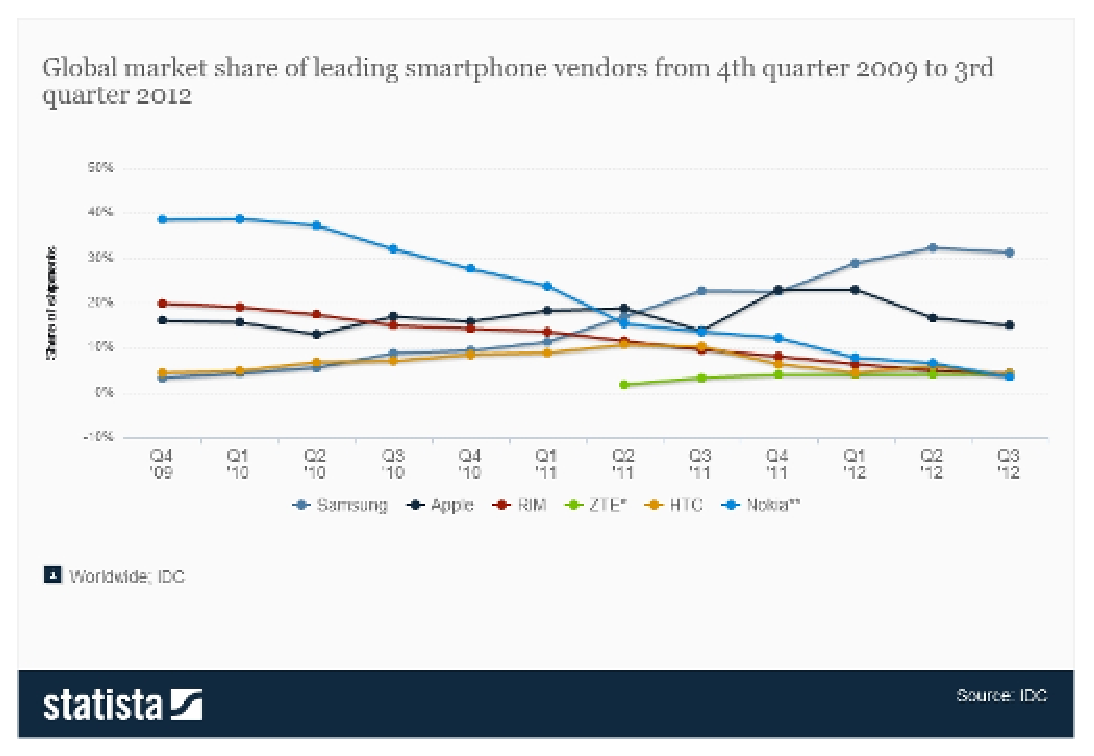
\includegraphics[width=1.0\textwidth]{smartphone_marketshare_vendors.eps}
\caption{Vývoj tržního podílu výrobců chytrých telefonů}
\label{fig:VyrobciSmartphoneRozsireni}
\end{figure}

Aktuální data z června roku 2012 ukazují zřetelnou převahu společnosti Samsung nad zbytkem trhu. Více než třetina dnes používaných smartphonů nese značku právě této společnosti. Oproti tomu zhruba polovičním podílem na trhu se může pochlubit společnost Apple. Původní hegemon – firma Nokia – nyní okupuje pouze lehce přes 6 \% tržního podílu.

\begin{figure}\centering
\includegraphics[width=0.6\textwidth]{smartphone_by_manufaturers.png}
\caption{Současný tržní podíl výrobců smartphonů na trhu}
\label{fig:VyrobciSmartphoneRozsireni2}
\end{figure}

\section{Přehled mobilních platforem}
Řada zákazníků při výběru nového chytrého telefonu dbá nejen na vzhled a hardwarové parametry, ale důležitou roli při konečném rozhodování hraje i operační systém, který na přístroji běží. Někteří výrobci se snaží s konkrétním operačním systémem spojit svou značku (Apple, Nokia), jiní naopak dávají zákazníkům na výběr různé modely s různými systémy (HTC, Samsung).

\subsection{iOS}
iOS je produktem společnosti Apple, která jím vybavuje své produkty iPhone, iPod i iPad. Poprvé byl uveden v roce 2007 spolu se smartphonem iPhone na konferenci Macworld \cite{apple_unveils_iPhone}. Od té doby je neustále vylepšován a v současné době se již nachází ve verzi 6. Od dob první verze se však uživatelské prostředí iPhonu mění jen pozvolna. Apple, narozdíl od konkurence v podobě Androidu a Windows Phone, neumožňuje použití systému iOS na zařízeních, které nevyrobila firma Apple.

Celý koncept systému iOS je úzce spjat s velkým displejem smartphonu iPhone. Ovládání celého prostředí je uživateli umožněno pomocí celé řady multi-dotykových gest. Mezi nejznámější prvky z prostředí systému iOS můžeme zařadit tzv. „Home screen“, který pomocí matice ikon usnadňuje uživateli spouštění nainstalovaných aplikací. Dále stojí za zmínku například notifikační centrum, hlasové ovládání Siri nebo Game center.

\subsubsection{Vývojářské technologie}
Aplikace pro systém iOS se programují primárně v jazyce Objective-C \cite{introduction_ios_development}. Objective-C je objektově orientovaný, reflektivní jazyk, v němž lze nalézt společné rysy se známým jazykem SmallTalk \cite{bp_dominik}. Poměrně složitá syntaxe Objective-C představuje značnou překážku pro začínající vývojáře, protože se výrazně liší od ostatních běžně používaných jazyků (například Javy v Androidu).

Díky kompilační struktuře naznačené v předchozí kapitole můžeme však místo Objective-C použít alternativní programovací jazyky, pokud k nim najdeme vhodný front-end. Toho využívá například projekt Monotouch, který vám umožňuje programovat nativní aplikace v C\# a frameworku .NET \cite{xamarin_monotouch}.

\subsubsection{Vývojářské nástroje}
Apple dává vývojářům k dispozici balík iOS SDK, který obsahuje široké spektrum nástrojů potřebných k tvorbě nativních aplikací pro systém iOS. Tento balík obsahuje například vývojové prostředí XCode, emulátor pro simulovaný běh aplikací na virtuálním zařízení, nástroj pro designování grafických prvků navrhované aplikace, offline verzi dokumentace a mnoho dalšího.

Pro vývoj aplikací pro iOS je nutné vlastnit počítač s operačním systémem Mac OS X. Toto je další poměrně značná překážka pro začínající vývojáře neboť počítače s tímto systémem jsou prozatím na trhu zastoupeny v marginální míře a konkurence v podobě Androidu umožňuje vyvíjet aplikace pro tento systém na libovolné platformě.  Pro publikování aplikací v tržišti App Store je navíc potřeba vlastnit placený vývojářský účet \cite{distribute_ios_app}.

\subsection{Android}
Operační systém Android byl původně vytvořen společností Android Inc., kterou v roce 2005 odkoupil gigant v oblasti internetového vyhledávání – firma Google \cite{google_buys_android}. Představení Androidu veřejnosti bylo úzce spjato se založením organizace Open Handset Alliance, která sdružovala výrobce software, hardware i telefonní operátory s cílem vyvinout otevřenou platformu a definovat nové standardy na poli mobilních telefonů \cite{android_announce}. Systém Android je šířen pod licencí Apache License a lze jej tedy označit za open-source software \cite{android_overview}.

Systém Android můžeme krom mobilních telefonů nalézt i na tabletech, chytrých televizích, herních konzolích a dalších zařízeních. Vysoká obliba Androidu mezi zákazníky pramení především z obrovského množství různých modelů, se kterými je tento systém na trhu nabízen. Vzhledem k otevřené licenci, pod kterou je systém šířen, je využíván širokým portfoliem výrobců, kteří tak ušetří za vývoj a správu vlastního systému.

Uživatelské rozhraní Androidu vzdáleně připomíná svého konkurenta iOS. Také zde najdeme „Home screen“, který je tvořen maticí ikon symbolizujících nainstalované aplikace. Stejně tak v Androidu můžeme nalézt třeba notifikační centrum. Od svých konkurentů se tato platforma odlišuje nepřeberným množstvím možností, jak upravit vzhled a chování systému.

\subsubsection{Vývojářské technologie}
Pro vývoj nativních aplikací se používá programovací jazyk Java. Podle společnosti TIOBE se jedná o druhý nejpoužívanější programovací jazyk na světě \cite{tiobe_software}. Java je objektově orientovaný jazyk se syntaxí blízkou jazykům C a C++.

Velkou výhodou Javy je její platformní nezávislost. Vlastní kód se totiž překládá do tzv. mezikódu, který je poté interpretován v rámci Java Virtual Machine \cite{understanding_jvm_internals}. Program napsaný v Javě je tak spustitelný na Windows, Mac OS X i Linuxu.

\subsubsection{Vývojářské nástroje}
Google, podobně jako Apple, připravil pro externí vývojáře balík všeho potřebného pro vývoj nativních aplikací, tzv. Android SDK. Ten obsahuje velmi populární vývojové prostředí Eclipse IDE obohacené o plugin ADT (Android Developer Tools). Toto rozšíření se stará o hlubokou integraci nástrojů samotného SDK do vývojového prostředí. Poskytuje tak GUI přístup například k debugovacím nástrojům (DDMS), návrhovým nástrojům pro uživatelské rozhraní, přístup a konfiguraci emulátorů a podobně.

Součástí SDK jsou samozřejmě i zdrojové kódy nejnovější verze systému Android a také obraz systému spustitelný v emulátoru. Nechybí ani podrobná dokumentace pro offline použití.

\subsection{Windows Phone}
Windows Phone vznikl ve společnosti Microsoft jako odpověď na úspěch iOS a Androidu. Předešlý systém z dílmy redmondské firmy, Windows Mobile, již nebyl lákavý pro výrobce zařízení s velkými dotykovými obrazovkami. Microsoft tak představil počátkem roku 2010 na Mobile World Congress v Barceloně zcela nový operační systém, který nesl označení Windows Phone 7 \cite{ms_announce_wp}. Jeho uživatelské rozhraní tvořené velkými barevnými interaktivními dlaždicemi se na první pohled velmi liší od iOS a Androidu, avšak většinu principů práce s dotykovými zařízeními zachovává. 

Společnost Microsoft narozdíl od Applu či Google doposud nevyrábí vlastní chytré telefony a tak přijetí nové platformy bylo čistě na vůli výrobců telefonů. Na tomto poli se nový systém střetával především s Androidem, který je výrobcům k dispozici zdarma, zatímco Microsoft požaduje za použití Windows Phone licenční poplatky. Jako svůj hlavní systém si Windows Phone zvolila společnost Nokia, která se spolu s ním snaží dobýt zpět své ztracené pozice na trhu s chytrými telefony.

Od roku 2010, kdy byl systém poprvé představen, byl již několikrát vylepšen mnoha aktualizacemi, které přinášely do systému nové funkce (např. multitasking). Dva roky po uvedení systému Windows Phone Microsoft oznámil vydání nové verze svého systému pod názvem Windows Phone 8, která přináší přepracované jádro a některé nové funkce \cite{ms_unveils_wp8}.

\subsubsection{Vývojářské technologie}
Pro vývoj aplikací pro systém Windows Phone 8 (ale i pro desktopové Windows) se primárně používá jazyk C\#. Tento jazyk byl vyvinutý spolu s frameworkem .NET firmou Microsoft. C\# je objektově orientovaný jazyk, u jehož syntaxe se Microsoft inspiroval u programovacích jazyků z rodiny C. Některé aspekty však přejal také z oblíbené Javy.

Framework .NET je komplexní balík knihoven a rozhraní určených pro vývoj, kompilaci a spouštění aplikací pro platformu Windows.

\subsubsection{Vývojářské nástroje}
Také pro platformu Windows Phone 8 existuje balík nástrojů určený pro vývoj nativních aplikací – Windows Phone 8 SDK. Jeho součástí je odlehčená verze Microsoft Visual Studia – Visual Studio Express 2012. Visual Studio je velmi oblíbené vývojové prostředí s širokým spektrem funkcí, jež sou vývojářům k dispozici. SDK obsahuje množství nástrojů pro návrh, testování, debugování a emulátory pro běh uživatelských aplikací.

\subsection{Firefox OS}
Firefox OS je mobilní operační systém, který je v současné době stále ještě ve vývoji a neběží tedy zatím na žádném reálně používaném zařízení. V této práci jej zmiňuji proto, že cíle, které si společnost Mozilla, jež stojí za tímto systémem, vytyčila, přímo korespondují s tématem této práce (více technických podrobností o Firefox OS naleznete v kapitole 2).

Vývoj systému Firefox OS byl oznámen v červnu 2011 v rámci komunity společnosti Mozilla. Celý projekt nesl kódové označení „Boot to Gecko“ a jeho cílem má být položení rovnítka mezi webové technologie a moderní mobilní telefony. V originální oznamovací zprávě se přímo říká \cite{booting_to_the_web}: „Chceme identifikovat překážky, které stěžují webovým vývojářům tvorbu aplikací, které budou v každém směru plnohodnotnými náhradami nativních aplikací pro platformy iOS, Android a WP7.“ První telefony s Firefox OS by se měly objevovat v prvním čtvrtletí roku 2013 \cite{ztes_first_firefoxos}.

\subsubsection{Aplikační technologie}
Protože nativní aplikace pro systém Firefox OS není nic jiného než „trochu vylepšená“ webová stránka (přesněji tzv. Open Web App \cite{faqs_mozilla}), nemůžeme od Firefox OS očekávat jakýkoliv proces kompilace.

Taková webová aplikace může samozřejmě fungovat jako běžná webová stránka uvnitř internetového prohlížeče. Uživatelé ovšem obvykle očekávají od mobilní aplikace více než od webové stránky. Aplikace ve Firefox OS běží mimo internetový prohlížeč. Ke svému běhu využívají tzv. Web runtime. Web runtime je software obsažený v internetovém prohlížeči, který však může běžet samostatně a zajišťuje celý životní cyklus aplikace od jejího spuštění, po obsluhu jejích požadavků až po její ukončení uživatelem \cite{apps_architecture}.

\subsubsection{Vývojářské technologie}
Jelikož jsme již naznačili, že pro vývoj nativních aplikací pro Firefox OS se používají pouze webové technologie dnes souhrnně (nesprávně?) označované jako rodina HTML5, do kterých řadíme:

\begin{enumerate}
	\item HTML5 jako značkovací jazyk ve své páté (dosud neoficiální) verzi obohacen o mnohé moderní funkce jako je geolokace, lokální databáze či nativní podpora pro přehrávání videa a audia.
	\item CSS3 pro definici vzhledu a částečně i chování uživatelského rozhraní aplikace.
	\item JavaScript je interpretovaný programovací jazyk, který se používá pro zajištění aplikační logiky. Jeho syntaxe se inspirovala u programovacích jazyků C/C++ a Java.
\end{enumerate}

\subsection{Vývojářské nástroje}
Mozilla nenabízí vývojářům aplikací pro Firefox OS (který stále ještě není v oficiálním prodeji) žádný balík se vším potřebným jako je tomu u jiných platforem. Důvodem pro tento fakt je pravděpodobně všudypřítomnost vývojářských nástrojů pro webové stránky/aplikace.

Přesto však firma Mozilla na konci roku 2012 vydala emulátor systému Firefox OS, na kterém mohou vývojáři testovat své aplikace aniž by museli vlastnit reálné zařízení. Firefox OS Simulator existuje pro Windows, Mac i Linux a lze jej dokonce získat i jako plugin do desktopové verze internetového prohlížeče Firefox \cite{announcing_fxOS_simulator}.

\subsection{Situace na trhu}
Podíváme-li se na aktuální situaci na trhu, můžeme jasně vidět, že na tomto poli nyní zcela zřetelně dominuje systém Android. Naopak dřívější hegemon Symbian, který poháněl zařízení společnosti Nokia, má již méně než 5 \% tržního podílu. iOS od Applu je pak druhým největším hráčem.

\begin{figure}\centering
\includegraphics[width=0.6\textwidth]{smartphone_by_platform.png}
\caption{Současný tržní podíl mobilních platforem}
\label{fig:MobilniPlatformyPodil}
\end{figure}

Další graf\ref{fig:MobilniPlatformyVyvoj} jasně ilustruje již zmíněné trendy. Můžeme zde vidět strmý propad Symbianu a naopak drtivý vzestup platformy Android, který od roku 2009 zaznamenala. 

\begin{figure}\centering
\includegraphics[width=1.0\textwidth]{graf_vyvoj_mobilnich_os.png}
\caption{Vývoj tržního podílu mobilních platforem}
\label{fig:MobilniPlatformyVyvoj}
\end{figure}

\section{Mobilní aplikace} \label{Sec:Aplikace}
Mobilní aplikaci definujeme jako samostatný software určený pro využití na smartphonech, tabletech a dalších přenosných zařízeních. Zpravidla jsou velmi úzce zaměřené na vykonání konkrétní činnosti a mají velmi málo funkcí (např. kalkulačka, internetový prohlížeč, čtečka RSS apod.).

Mobilní aplikace jsou převážně distribuovány přes takzvaná „tržiště“, kde uživatel najde kategorizovaný přehled aplikací, které si může pro svou platformu stáhnout (více o tržištích v podkapitole XY). Některé platformy podporují i možnost stahování mobilních aplikací prakticky odkudkoliv, například z webových stránek vývojáře, který aplikaci vytvořil (Android).

\subsection{Rozdělení mobilních aplikací}
Pro rozdělení mobilních aplikací můžeme využít v zásadě dva přístupy. Jedním z nich je rozdělit aplikace podle účelu, za nímž byly stvořeny. Další možností je potom rozdělit takové aplikace dle technologie, pomocí které byly vytvořeny.

\subsubsection{Rozdělení dle účelu}
Při rozdělování aplikací dle účelu se musíme zaměřit na oblast činnosti, kterou má daná aplikace svému uživateli zpříjemnit. Níže jsem provedl jejich rozdělení dle účelu, při jehož tvorbě jsem vycházel z kategorizace, kterou pro rozdělení aplikací používají oficiální tržiště pro platformy iOS a Android.

\begin{enumerate}
	\item Hry
	\item Sociální sítě
	\item Multimédia – například aplikace na úpravu fotografií, přehrávání videa nebo hudby.
	\item Produktivita – GTD aplikace, time tracking apod.
	\item Komunikace – IM komunikátory, SMS aplikace apod.
	\item Doprava – GPS navigace, mapy apod.
	\item Cestování
	\item Kancelářské – zjednodušené verze kancelářských balíků, správa financí apod.
	\item Zábava
	\item. Nakupování – tipy, slevy apod.
	\item Informační – čtení zpráv, vzdělávání, počasí.
	\item Úpravy systému – rozšířené možnosti nastavení a úprav vzhledu.
	\item Životní styl – zdraví, jídlo.
	\item Sport – živé výsledky, informace.
\end{enumerate}

\subsection{Dle technologie}
\subsubsection{Nativní aplikace}
Již ze slova „nativní“ v názvu této sekce plyne, že půjde o technologii, která je nějakým způsobem přirozená. V našem případě je to přirozenost technologie a chování aplikace k dané platformě. Pro vývoj mobilní aplikace pro konkrétní operační systém tedy používáme určitý programovací jazyk a určité nástroje. 

Nativní aplikace se většinou vyznačují dobrým výkonem a širokým spektrem funkcí. Vývojáři nativních aplikací mají totiž přístup k drtivé většině hardwarových i softwarových funkcí telefonu. I vzhled nativních aplikací je přesně takový, jaký ho uživatel očekává. Některé platformy mají totiž velmi striktní požadavky na vzhled jednotlivých ovládacích prvků (tlačítek, přechodů apod.) a nevyhovující aplikace vůbec nepřipouští na svá tržiště.

Nativní aplikace jsou většinou distribuovány přes oficiální tržiště konkrétní platformy. U operačního systému Android však můžeme pozorovat i jiné cesty, kterými uživatelé aplikace získávají (z webových stránek, neoficiální tržiště apod.). Více o vývoji nativních aplikací pro jednotlivé platformy si řekneme v kapitole 2.

\subsubsection{Webová aplikace}
Aplikaci označujeme jako webovou, pokud bylo při jejím vývoji použito tzv. webových technologií (např. HTML či JavaScript). Webová aplikace ke svému běhu potřebuje internetový prohlížeč nebo jeho jádro. Všeobecná rozšířenost webových aplikací pramení právě z tohoto faktu. Internetový prohlížeč je totiž předinstalován na všech známých operačních systémech (desktopových i mobilních) a díky tomu je velmi široce rozšířený.

V prostředí mobilních telefonů nacházejí webové aplikace uplatnění zejména díky nízkým nákladům na vytvoření a jejich multiplatformnosti. Webová aplikace na mobilním telefonu může mít buď formu webové stránky uzpůsobené pro zobrazení na malých displejích či offline aplikace, která ke svému běhu nevyžaduje internetové připojení.

Velkým nedostatkem, jímž webové aplikace trpí, je jich omezená funkcionalita. Webové aplikace nemohou přistupovat k žádným specifickým funkcím telefonu vyjma samotného internetového prohlížeče. Proto se webové aplikace využívají především jako zobrazovač obsahu, který je formátován pro snadnou konzumaci na mobilním telefonu.

\subsubsection{Hybridní aplikace}
Definice hybridních aplikací není zatím úplně přesně vymezená. Pokud bych se měl pokusit takovou aplikaci definovat, tak se jedná o aplikaci, pro jejíž vývoj bylo použito převážně webových technologií, avšak hybridní aplikace umožňuje uživateli využívat některé hardwarové i softwarové funkce telefonu stejně, jako by se jednalo o aplikaci nativní.

Hybridní aplikace se navenek tváří stejně jako aplikace nativní, takže většinou splňují všechny požadavky, které si kladou oficiální tržiště. Uživatel si pak takovou aplikaci stáhne aniž by věděl, že nebyla vyvinuta v nativním kódu. Více o hybridních aplikacích se dozvíte v kapitolách 3, 4 a 5. % TODO reference

\subsection{Popularita mobilních aplikací}
Chytré telefony byly ve svých počátcích populární zejména díky přístupu na internet přes webový prohlížeč. Dnes však tomuto světu začínají pozvolna vládnout aplikace. Průměrný uživatel smartphonu měl v roce 2012 na svém zařízení nainstalováno 41 aplikací, přičemž o rok dříve to bylo jen 32 \cite{mobile_app_usage_statistics}. Tento strmý vzestup dobře ilustruje i poměr, v jakém uživatelé využívají internetový prohlížeč oproti staženým aplikacím. V roce 2012 bylo poprvé zaznamenáno, že uživatelé používali pro přístup k obsahu více stažené aplikace než internetový prohlížeč. V květnu 2012 byl tento poměr 51,1 \% ku 49,8 \% ve prospěch aplikací \cite{comscore_report_may}.

Popularita mobilních aplikací je založena na několika faktorech. Jedním z nich je nepopiratelně jejich nízká cena. Mobilní aplikace v Apple App Store stojí v lednu 2013 průměrně 1,61 \$ \cite{app_store_metrics}. Za takto nízkou cenu se většině uživatelů vyplatí, především z důvodu pohodlí, aplikaci zakoupit, než podstupovat poměrně složitý proces odemčení telefonu a následného nahrávání aplikací nelegálně stažených z internetu. Tento fakt je v ostrém kontrastu s prostředím desktopových aplikací, které často stojí tisíce korun a pro mnoho lidí jsou z tohoto důvodu nedostupné a ti se poté uchylují k pořizování pirátských kopií tohoto software.

Dalším faktorem, který zapříčiňuje popularitu aplikací, je nepochybně pohodlí při jejich obstarávání. Uživatelé platformy Windows byli po léta zvyklí, že software pro svůj počítač museli stahovat z různých (často pochybných) zdrojů. Vyžadovalo to od nich zvýšené úsilí s často neuspokojivým výsledkem. Oficiální distributoři mobilních aplikací se snaží toto úsilí redukovat na minimum. Každá platforma má své oficiální tržiště, kde dělí uživatele od získání jeho aplikace doslova jediný klik. Díky tomu mohou vývojáři oslovovat obrovskou masu uživatelů a držet tak cenu svých aplikací velmi nízko.

Třetím a možná nejdůležitějším faktorem je přirozeně velice příznivé prostředí pro vývojáře. Společnosti stojící za vývojem jednotlivých platforem si svou komunitu developerů značně hýčkají. Krom pečlivé dokumentace mají připravené i specializované nástroje, kterými vývoj nativních aplikací pro své platformy usnadňují. Navíc díky výše zmíněné jednoduchosti finální distribuce se vývojář nemusí příliš zabývat s marketingem kolem své aplikace. O příznivém prostředí pro vývojáře svědčí i fakt, že od spuštění Apple App Store jim bylo za prodej placených aplikací vyplaceno více než 5 miliard dolarů \cite{comscore_report_may}.

Samostatným segmentem trhu jsou firmy a jejich vztah k mobilním aplikacím. Velké i malé firmy používají aplikaci ke komunikaci se svými zákazníky a to z několika hledisek. Jednak je to pro ně skvělý marketingový kanál. Přes specializované aplikace ke svým produktům či službám mohou oslovovit cílovou skupinu, která má o jejich produkty zájem a nabídnout jim něco navíc. Nenahánějí tedy zajíce v pytli, ale cílí na uživatele, kteří projevili o jejich aplikaci (a potažmo produkt) zájem. Mohou jim pak šít nabídky přímo na míru, poskytovat speciální slevy a podobně. Zajímavým benefitem pro uživatele je i poskytnutí podrobných informací o produktech, usnadnění jejich nákupu či komunikace s firmou. Podle některých předpovědí bude mobilní aplikace pro firmy do budoucna stejně důležitý komunikační kanál, jakou je dnes třeba e-mailová adresa či telefon \cite{forbes_business_checklist}.
% TODO dodělat chybějící literaturu